%-------------------------
% Resume in Latex
% Author : Jonathan Oktaviano Frizzy
% License : MIT
%------------------------

\documentclass[letterpaper,11pt]{article}

\usepackage{latexsym}
\usepackage[empty]{fullpage}
\usepackage{titlesec}
\usepackage{marvosym}
\usepackage[usenames,dvipsnames]{color}
\usepackage{verbatim}
\usepackage{enumitem}
\usepackage[hidelinks]{hyperref}
\usepackage{fancyhdr}
\usepackage[english]{babel}
\usepackage{tabularx}
\usepackage{hyphenat}
\usepackage{fontawesome}
\usepackage{graphicx}
\input{glyphtounicode}


%---------- FONT OPTIONS ----------
% sans-serif
% \usepackage[sfdefault]{FiraSans}
% \usepackage[sfdefault]{roboto}
% \usepackage[sfdefault]{noto-sans}
% \usepackage[default]{sourcesanspro}

% serif
% \usepackage{CormorantGaramond}
% \usepackage{charter}


\pagestyle{fancy}
\fancyhf{} % clear all header and footer fields
\fancyfoot{}
\renewcommand{\headrulewidth}{0pt}
\renewcommand{\footrulewidth}{0pt}

% Adjust margins
\addtolength{\oddsidemargin}{-0.5in}
\addtolength{\evensidemargin}{-0.5in}
\addtolength{\textwidth}{1in}
\addtolength{\topmargin}{-.5in}
\addtolength{\textheight}{1.0in}

\urlstyle{same}

\raggedbottom
\raggedright
\setlength{\tabcolsep}{0in}

% Sections formatting
\titleformat{\section}{
  \vspace{-4pt}\scshape\raggedright\large
}{}{0em}{}[\color{black}\titlerule \vspace{-5pt}]

% Ensure that generate pdf is machine readable/ATS parsable
\pdfgentounicode=1

%-------------------------
% Custom commands

\newcommand{\resumeItem}[1]{
  \item\small{
    {#1 \vspace{-2pt}}
  }
}


\newcommand{\resumeSubheading}[4]{
  \vspace{-2pt}\item
    \begin{tabular*}{0.97\textwidth}[t]{l@{\extracolsep{\fill}}r}
      \textbf{#1} & #2 \\
      \textit{\small#3} & \textit{\small #4} \\
    \end{tabular*}\vspace{-7pt}
}


\newcommand{\resumeSubSubheading}[2]{
    \vspace{-2pt}\item
    \begin{tabular*}{0.97\textwidth}{l@{\extracolsep{\fill}}r}
      \textit{\small#1} & \textit{\small #2} \\
    \end{tabular*}\vspace{-7pt}
}


\newcommand{\resumeEducationHeading}[6]{
  \vspace{-2pt}\item
    \begin{tabular*}{0.97\textwidth}[t]{l@{\extracolsep{\fill}}r}
      \textbf{#1} & #2 \\
      \textit{\small#3} & \textit{\small #4} \\
      \textit{\small#5} & \textit{\small #6} \\
    \end{tabular*}\vspace{-5pt}
}


\newcommand{\resumeProjectHeading}[2]{
    \vspace{-2pt}\item
    \begin{tabular*}{0.97\textwidth}{l@{\extracolsep{\fill}}r}
      \small#1 & #2 \\
    \end{tabular*}\vspace{-7pt}
}


\newcommand{\resumeOrganizationHeading}[4]{
  \vspace{-2pt}\item
    \begin{tabular*}{0.97\textwidth}[t]{l@{\extracolsep{\fill}}r}
      \textbf{#1} & \textit{\small #2} \\
      \textit{\small#3}
    \end{tabular*}\vspace{-7pt}
}

\newcommand{\resumeSubItem}[1]{\resumeItem{#1}\vspace{-4pt}}

\renewcommand\labelitemii{$\vcenter{\hbox{\tiny$\bullet$}}$}

\newcommand{\resumeSubHeadingListStart}{\begin{itemize}[leftmargin=0.15in, label={}]}
\newcommand{\resumeSubHeadingListEnd}{\end{itemize}}
\newcommand{\resumeItemListStart}{\begin{itemize}}
\newcommand{\resumeItemListEnd}{\end{itemize}\vspace{-5pt}}

%-------------------------------------------
%%%%%%  RESUME STARTS HERE  %%%%%%%%%%%%%%%%%%%%%%%%%%%%


\begin{document}

% HEADING
\begin{tabularx}{\textwidth}{@{}l X@{}}
    \begin{minipage}[c][6em][t]{0.15\textwidth} % 6em adalah tinggi vertikal ruangan untuk gambar
        \vspace{-1 em} % Ruang tambahan sebelum gambar
        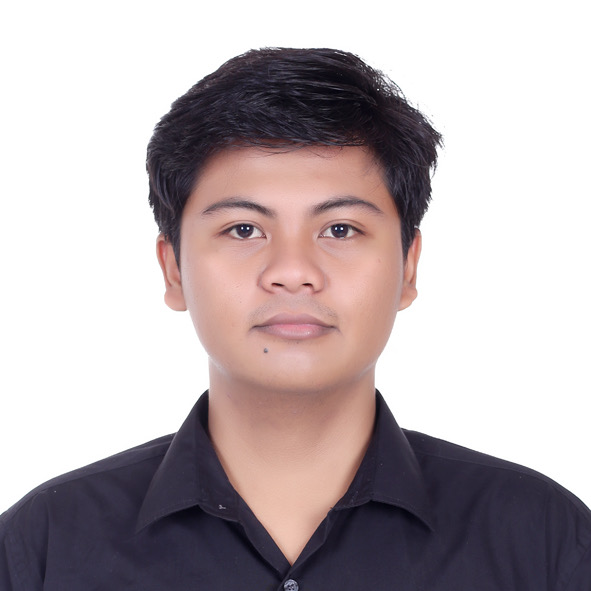
\includegraphics[width=\textwidth]{fix.jpg} % Mengatur lebar gambar agar sesuai
    \end{minipage}
    \hspace{5 mm} % Menambahkan spasi antara gambar dan konten di kanan
    & \begin{tabular}{@{}l@{}}
        \textbf{\Huge \scshape Jonathan Oktaviano Frizzy} \\[0.8em] % Jarak setelah nama
        \faMobile \hspace{.5pt} \href{https://wa.me/081357473781}{+62 813 5747 3781}
        $|$
        \faAt \hspace{.5pt} \href{mailto:jonathanoktavianofrizzy@gmail.com}{jonathanoktavianofrizzy@gmail.com} \\[0.1em] % Mengatur jarak antara baris
        \faLinkedinSquare \hspace{.5pt} \href{https://linkedin.com/in/jonathan-oktaviano/}{jonathan oktaviano frizzy}
        $|$
        \faGithub \hspace{.5pt} \href{https://github.com/robotjaol}{GitHub}
        $|$
        \faGlobe \hspace{.5pt} \href{https://robotjaol.vercel.app/}{Portfolio}
        $|$
        \faMapMarker \hspace{.5pt} \href{https://maps.app.goo.gl/3KcJKWS8gMk1GiZMA}{Surabaya, Indonesia} \\
    \end{tabular}
\end{tabularx}
\vspace{.2em}

%----------- EDUCATION -----------

% \section{Education}
%   \vspace{3pt}
%   \resumeSubHeadingListStart
    
%     \resumeEducationHeading
%       {Institut Teknologi Sepuluh Nopember}{Surabaya, Indonesia}
%       {1nd Year in Electrical Automation Engineering; \textbf{GPA: 3.49/4.00}}{Jul 2022 \textbf{--} Apr 2023}
      
    
  
%   \resumeSubHeadingListEnd

 \section{Education}
   \vspace{3pt} 
    \resumeSubHeadingListStart

       \resumeEducationHeading
         {Institut Teknologi Sepuluh Nopember}
         {Surabaya, Indonesia}
         {3nd Year in D4 Automation Electronic Engineering}
         {GPA: 3.55/4.00}
         {Jul 2022 -- Present}
  
    \resumeSubHeadingListEnd

%----------- EXPERIENCE -----------

\section{Experience}
  \vspace{3pt}
  \resumeSubHeadingListStart

    \resumeSubheading
      {PLC and Supervisory Control System Laboratory ITS}{Surabaya, Indonesia}
      {Member}{Dec 2022 \textbf{--} Present, Full-time}
        \resumeItemListStart
            \resumeItem{Contributed to 3 key projects over 3 semesters, including the application of Yolo for machine vision, embedded systems development using STM32, and a website monitoring system.}
            \resumeItem{Co-authored academic papers and contributed to intellectual property rights filings for automation systems.}
            \resumeItem{Focused on industrial automation development, machine vision, automation electricity, and project-based learning with industry collaboration.}
        \resumeItemListEnd

    \resumeSubheading
      {Barunastra ITS}{Surabaya, Indonesia}
      {Electrical Designer}{Dec 2022 \textbf{--} Present, Full-time}
        \resumeItemListStart
            \resumeItem{Developed an emergency control breaker system using two parameters (Signal and Power), remotely controlled via radio frequency for enhanced safety.}
            \resumeItem{Managed over 50 types of components and more than 200 individual parts to optimize electrical performance and compliance with safety standards.}
            \resumeItem{Designed and implemented power electronics circuits, analog systems, and embedded systems based on STM32 for various autonomous vehicle projects.}
        \resumeItemListEnd
    
    \resumeSubheading
      {Digital Talent Scholarship KOMINFO}{Surabaya, Indonesia}
      {Teaching Assistant}{Jan 2023 \textbf{--} Jun 2023, Part-time}
        \resumeItemListStart
            \resumeItem{Supported 100 participants in the Junior Website Developer program, guiding them through coding exercises and project development.}
            \resumeItem{Managed attendance data for each session and facilitated learning outcomes for participants.}
            \resumeItem{Evaluated 30 final projects, providing feedback and assigning assessment points for feature implementations.}
        \resumeItemListEnd


    \resumeSubheading
      {PT. Pertamina Trans Kontinental}{Cilacap, Indonesia}
      {Electrical Engineer}{Jun 2023 \textbf{--} Dec 2023, Full-time}
        \resumeItemListStart
            \resumeItem{Designed and developed energy-efficient electrical systems, leading to a 30\% improvement in energy savings for oil navigation vessels through the adoption of optimized battery systems.}
            \resumeItem{Led a team of 5 engineers in the integration of communication tools and power management solutions to ensure seamless operation on board vessels.}
            % \resumeItem{Provided technical expertise in onboard communication systems and electrical architecture.}
    \resumeItemListEnd
    
    \resumeSubheading
      {Bioinformatics Study Club ITS}{Surabaya, Indonesia}
      {Vice Chairman}{Jun 2023 \textbf{--} Present, Part-time}
        \resumeItemListStart
            \resumeItem{Assisted the Chairman in overseeing club operations, organizing research projects, workshops, and events.}
            \resumeItem{eading a core team of 20 members and overseeing over 30 members in total, ensuring smooth operations and successful execution of research projects, workshops, and events.}
        \resumeItemListEnd

    \resumeSubheading
      {KKN Tematik Institut Teknologi Sepuluh Nopember}{Surabaya\textbf{--}Sidoarjo, Indonesia}
      {Project Leader}{Aug 2023 \textbf{--} Oct 2023, Part-time}
        \resumeItemListStart
            \resumeItem{Led a team of 6 members in the Smart Integrated Water Quality Monitoring System project, responsible for timeline, finances, and logistics.}
            \resumeItem{Developed a monitoring device using 5 sensors with a 90\% accuracy rate, capable of maneuvering across various water bodies.}
            \resumeItem{Designed the installation scheme for sensing components, actuators, and radio transmitters, with data accessible from anywhere via a web interface.}
        \resumeItemListEnd
        
    \resumeSubheading
      {PT. Innoveam}{Surabaya, Indonesia}
      {Electrical Engineer}{Jul 2024 \textbf{--} Aug 2024, Full-time}
        \resumeItemListStart
            \resumeItem{Led the creation of detailed electrical schematics for each robot, optimizing the layout and integration of components to ensure efficient power distribution and control.}
            \resumeItem{Conducted comprehensive troubleshooting and diagnostics, identifying and resolving electrical issues that could affect the robots' precision and operational reliability.}
            \resumeItem{Programmed and controlled the robots’ individual components using microcontrollers, ensuring seamless communication between sensors, motors, and actuators to achieve high-accuracy target engagement.}
    \resumeItemListEnd

      %    \resumeSubheading
      % {Wirausaha Merdeka ITS}{Surabaya, Indonesia}
      % {Electronics Engineer}{June 2023 \textbf{--} Oct 2023, Part-time}
      %   \resumeItemListStart
      %       \resumeItem{I designed and developed the electrical system for the "Beginner Kit Electronics" product using Autodesk Fusion 360 for the design and Proteus for circuit simulation. Additionally, I participated in business management training to meet specific business criteria and fulfill the requirements for the Free Entrepreneurship activity evaluation.  \href{https://www.youtube.com/watch?v=fzd8DhDGEHg}{\color{blue}Here is the documentation}.}
      %   \resumeItemListEn
    
  \resumeSubHeadingListEnd



%----------- AWARDS & ACHIEVEMENTS -----------

\section{Awards \& Achievements}
  \vspace{2pt}
  \resumeSubHeadingListStart
    \small{\item{
        \textbf{Autonomy Challenge at International Roboboat Competition:}{ - 3rd place by integrating and coordinating all electronic components in 'Nala Proteus V.2,' including PCB, sensors, and actuators. Developed electrical and communication architecture, implemented with a success rate of 90\% {(Feb 2024) $|$ \href{https://robonation.org/app/uploads/sites/3/2023/02/TDR_Institut-Teknologi-Sepuluh-Nopember_RB2023.pdf}{\color{blue}Paper}.} \\ \vspace{3pt}
        
        \textbf{Autonomy Challenge at International Roboboat Competition:}{ - 1st place, Led the development of the electrical architecture and battery management for ‘Nala Proteus,’ ensuring seamless integration of PCB and sensor systems. {(Mar 2023) $|$ \href{https://robonation.org/app/uploads/sites/3/2023/12/TDR_ITS-Barunastra_RB2024.pdf}{\color{blue}Paper}.} \\ \vspace{3pt}
        
        \textbf{Autonomous Tourism Surface Vehicle Prototype Contest, (KKCTBN):}{ - 1st place Contributed to the electrical design of ‘Nala Athena’ Autonomous Tourism Surface Vehicle, securing top placement. (Oct 2023)} \\ \vspace{3pt}
        
        \textbf{LKS Nasional Mobile Robotic:}{ - 3rd place Developed a service robot using MyRIO and National Instruments controller, with integrated sensors for navigation and obstacle detection. (Oct 2022)} \\ \vspace{3pt}
        
        % \textbf{SMK Sore Tulungagung Award:}{ Graduated as the highest ranked student.(Jun 2022)}
    }}}}
\resumeSubHeadingListEnd



%----------- PROJECTS -----------

\section{Projects}
    \vspace{3pt}
    \resumeSubHeadingListStart            
      \resumeProjectHeading
            {\textbf{PT. Robo Marine Indonesia "Autonomous Modular USV HydroOceanography"} $|$ \emph{\href{https://www.linkedin.com/feed/update/urn:li:activity:7245271363135922177/}{\color{blue}Article}}}{}
          \resumeItemListStart
            \resumeItem{Served as an electrical staff for the Autonomous Modular Unmanned Surface Vehicle (USV) HydroOceanography project. Responsible for designing and implementing the power schematic and wiring system, including creating the PCB for powering the entire USV. Collaborated with a team of three to ensure proper power distribution and functionality across all components, from automation systems to navigation. Participated in the physical installation of wiring and components, ensuring seamless integration and operational efficiency.}
          \resumeItemListEnd

     \resumeProjectHeading
        {\textbf{PT. Pertamina Trans Kontinental "Oil Navigating Ship"} $|$ \emph{\href{https://www.linkedin.com/in/jonathan-oktaviano/details/projects/}{\color{blue}LinkedIn Experience}}}{}
          \resumeItemListStart
            \resumeItem{Acted as the electrical and mechanical consultant, responsible for designing both communication and electrical diagrams for oil navigation vessels. Spearheaded strategic recommendations on system integration, leading to a 30\% energy efficiency improvement through optimized battery management and ship maneuvering processes.}
          \resumeItemListEnd
          
    \resumeSubHeadingListEnd

    
%----------- SKILLS -----------

\section{Skills}
  \vspace{2pt}
  \resumeSubHeadingListStart
    \small{\item{
        
        \textbf{Languages:}{ C/C++, C\#, Python, JavaScript, PHP, LabVIEW, MATLAB} \\ \vspace{3pt}
        
        \textbf{Technologies:}{ Flask, Streamlit, Node.js, React.js, Git, RabbitMQ, OpenCV, PyTorch, Mediapipe, TensorFlow, Arduino, ESP32, ESP8266, STM32, PLC Omron, PLC Mitsubishi, ROS2, KiCAD, Fusion360 CAD, Altium Designer} \\ \vspace{3pt}
        
        \textbf{Methodologies:} {OOP, Functional Programming, Kinematics, PID, Neural Network, CNN} \\ \vspace{3pt}
        
    }}
  \resumeSubHeadingListEnd


%----------- RELEVANT COURSEWORK -----------

% \section{Relevant Coursework}
%   \vspace{2pt}
%   \resumeSubHeadingListStart
%     \small{\item{
%         \textbf{Major coursework:}{ Materials Science, Electrical Circuits I-II, Digital System Design, Numerical Methods, Probability Theory, Electronics I-II, Signals and Systems, Electromagnetic Field Theory, Energy Conversion, System Dynamics and Control, Communication Engineering, Pattern Recognition, Introduction to Digital Signal Processing, Introduction to Digital Communications, Introduction to Database Systems, Introduction to Image Processing, Machine Vision} \\ \vspace{3pt}

%         \textbf{Minor coursework:}{ Discrete Computational Structures, Introduction to Object-Oriented Programming, Data Structures and Algorithms, Computer Organization, Fundamentals of Software Engineering}
%     }}
%   \resumeSubHeadingListEnd



%----------- CERTIFICATES -----------

\section{Certificates}
\resumeSubHeadingListStart
    \resumeOrganizationHeading
      {Project Manager by Google}{Mar 2024}{Foundation Project Management \href{https://www.coursera.org/account/accomplishments/verify/FUGNKUSUYHBA}{\color{blue}Certificate}.}

    \resumeOrganizationHeading
      {Artificial Intelligence for Business by NASBA}{Mar 2024}{Introduction to Artificial Intelligence \href{https://www.linkedin.com/in/jonathan-oktaviano/details/certifications/1710528282367/single-media-viewer/?profileId=ACoAAEB2k00Bw-v1yxcDJJYIGidC5SNJ_jZ5UHg}{\color{blue}Certificate}.}

    \resumeOrganizationHeading
      {CS50's Introduction to Artificial Intelligence with Python}{Aug 2024}{Artificial Intelligence (AI) and Python (Programming Language) by Harvard University. \href{https://www.linkedin.com/in/jonathan-oktaviano/details/certifications/}{\color{blue}Certificate}.}

  \resumeSubHeadingListEnd



%----------- ORGANIZATIONS -----------

\section{Organizations}
  \resumeSubHeadingListStart

    % \resumeOrganizationHeading
    %   {UKM Robotika ITS}{Oct 2022 -- Present}{Member}
      
    \resumeOrganizationHeading
      {Barunastra ITS}{Dec 2022 -- Present}{Expert Staff Electrical Division}

    \resumeOrganizationHeading
      {Bioinformatics Study Club ITS}{May 2024 -- Present}{Vice Chairman}

  \resumeSubHeadingListEnd



%----------- HOBBIES -----------

% \section{Hobbies}
  % \resumeSubHeadingListStart
    % \small{\item{Basketball, Swimming, Fitness, Eight-ball, Horology}}
  % \resumeSubHeadingListEnd



%----------- REFERENCES -----------

% \section{References}
  % \vspace{2pt}
  % \resumeSubHeadingListStart
    % \item{References available upon request.}
  % \resumeSubHeadingListEnd



%-------------------------------------------
\end{document}